\documentclass[12pt, a4paper]{article}
\title{Relazione progetto ROOT} %argomento
\date{}
\author{Stella Baldrati, Giacomo Errani, Riccardo Giuliani}

\setlength{\parindent}{0pt}
\usepackage{setspace}
\usepackage[margin=0.5in]{geometry}
\usepackage{float}
\usepackage{amsfonts}
\usepackage{pdfpages}
\usepackage{verbatim}
\usepackage[utf8]{inputenc}
\usepackage{subcaption}
\usepackage{graphicx}

%\usepackage{siunitx} 
%\sisetup{
  %round-mode          = places, % Rounds numbers
 % round-precision     = 2, % to 2 places
%}

\graphicspath{ {./images} } %cartella immagini, separata dalla cartella files

\usepackage{listings}
\usepackage{xcolor}


\begin{document}

\maketitle

\section{Introduzione}
%%inserire un po' di teoria alla base e sintetizzare tutto il contenuto come in un abstract

L'approccio sperimentale utilizzato in fisica delle particelle per studiarne proprietà e interazioni si basa sullo studio dei prodotti di collisioni ad alta velocità. In seguito a questi urti, si genera un numero di particelle di varie tipologie stimato in $10^2-10^4$ per ogni evento di collisione. 
\newline
Le particelle più stabili sono direttamente rilevabili e si possono classificare tramite analisi della traiettoria. Vi sono però anche particelle instabili, dette risonanze, che decadono in tempi brevissimi e non sono direttamente rilevabili; per studiarle si rende necessario analizzare i prodotti dei loro decadimenti, che generalmente sono particelle sufficientemente stabili.
\newline
Il programma qui illustrato simula eventi di collisione e genera prodotti assimilabili a quelli ottenibili tramite un acceleratore. Analizza poi le particelle generate ed elabora i decadimenti, rappresentandone quantità e distribuzioni tramite grafici ROOT. 

In particolare, consente di studiare il comportamento della risonanza K*, cercandone il picco caratteristico di massa invariante dovuto ai prodotti del suo decadimento nel segnale di fondo.

\section{Struttura del codice}
%quali classi sono state implementate, con che funzione,
%quali meccanismi di reimpiego di codice sono stati usati, e perchè

\subsection{Programma di generazione}

Sono state implementate le seguenti classi:

\begin{enumerate}
\item ParticleType: rappresenta una generica particella stabile categorizzandola mediante massa, carica e tipologia, e fornisce un'interfaccia per accedere a questi dati. Implementa inoltre una funzione \verb!GetWidth! che fornisce una larghezza di risonanza nulla, necessaria per poter utilizzare il polimorfismo dinamico. 
Definisce un enum che identifica i tipi di particelle utilizzabili, poi associati alle istanze di ParticleType.

\item ResonanceType: classe derivata di ParticleType, rappresenta il fenomeno di risonanza per una particella instabile con l'attributo larghezza di risonanza e reimplementa \verb!GetWidth! per restituire il valore corretto. 

\item Particle: rappresenta una particella della simulazione, mediante il tipo e la quantità di moto. 
Fornisce dei metodi per accedere agli attributi della particella, per calcolare la massa invariante ed elaborare un decadimento (funzione \verb!Decay2Body!).
Definisce un vettore statico (\verb!fParticleTypes!) che memorizza i tipi di particelle, associati alle singole istanze mediante l'attributo \verb!fParticleName!.

\item ProportionGenerator: class template che implementa il generatore secondo definite proporzioni. 
\item ParticleGenerator: oggetto funzione che incapsula la generazione delle particelle. 
Fornisce un \verb!operator()! per eseguire la generazione e una funzione \verb!loadParticles()! per caricare i parametri dei tipi di particelle nel vettore \verb!fParticleTypes!.

\item ParticleStorage: struct serializzabile che memorizza i vari istogrammi, generata da ParticleGenerator. 

\end{enumerate}

\subsection{Programma di analisi}

\begin{enumerate}
\item ParticleAnalyser: incapsula la lettura del file root (con controllo integrità dei dati mediante un cast dinamico) nel costruttore. Fornisce un metodo \verb!GetData! per accedere ai dati, una funzione di analisi dei segnali dei decadimenti (\verb!GetDecaymentSignal!) e una di analisi delle distribuzione di generazione (\verb!GetGenerationFits!). 

\item AnalyserGraphics: incapsula la presentazione dei dati, crea i canvas, configura lo stile, disegna istogrammi e fit.


\end{enumerate}

\subsection{Tecniche di reimpiego del codice}
%note su cosa scrivere: tecniche oop, incapsulamento, uso della classe proportion generator, implementare la funzionalità comune in classi e usando funzioni generiche, nascondendo i dettagli implementativi
Abbiamo usato le tecniche della programmazione OOP per separare i dettagli implementativi dall'interfaccia, incapsulando le funzioni e rendendo il tutto modulare.
\newline

In particolare, la classe \verb!ProportionGenerator! si adatta a generare qualsiasi tipo di oggetto, note le istanze generabili e le probabilità.
\newline

Infine, l'uso del polimorfismo dinamico nelle classi \verb!ParticleType! e \verb!ResonanceType! consente di gestire le particelle stabili e instabili con puntatori di tipo \verb!ParticleType!, trattandole come se fossero dello stesso tipo.

\section{Generazione}
% specifichiamo che si tratta di eventi separati e non tutte insieme

Sono stati elaborati 10$^5$, in ciascuno dei quali sono state generate 10$^2$ particelle, secondo definite proporzioni, di tipo pione($\pi$), kaone(K), protone(P) e kaone instabile(K*):

\begin{itemize}

\item Tutti i tipi di particelle si presentano nella doppia forma positiva (+) e negativa (-). 

\item La composizione del campione è stata così generata: 40\% pioni positivi, 40\% pioni negativi, 5\% kaoni positivi, 5\% kaoni negativi, 4.5\% protoni positivi, 4.5\% protoni negativi, e 1\% kaoni instabili.

\item Le proprietà cinematiche delle particelle (angolo polare, angolo azimutale, modulo della quantità di moto) sono state generate tramite la generazione Monte Carlo di ROOT, utilizzando le funzioni \verb!TRandom::Rndm()!, 
\verb!TRandom::Uniform()!,\verb!TRandom::Exp(double mean)!.

\end{itemize}

\subsection{Elaborazione dei decadimenti}
In ogni evento si generano 1-2 K*, il cui decadimento è elaborato in fase di generazione.
Da una K* si possono ottenere o una coppia Pione+/Kaone- o Pione-/Kaone+, ciascuna con probabilità del 50\%.


\section{Analisi}
%Discutere la congruenza delle distribuzioni osservate con i dati in input
%alla generazione, spiegare brevemente l’approccio seguito per estrarre il segnale
%della risonanza
Riportiamo le tabelle delle occorrenze dei tipi di particelle, distribuzione di generazione dei parametri cinematici e segnale della K*.

\begin{table}[H]
  \begin{center}
    \caption{Abbondanza delle particelle.}
    \label{tab:table1}
    \begin{tabular}{c|c|c} % 
      \textbf{Specie} & 
      \textbf{Occorrenze osservate ($10^3$)} & 
      \textbf{occorrenze attese ($10^3$)}\\
      
      \hline
      $\pi$+ & 4000 $\pm$ 2 & 4000\\
      $\pi$- & 4000 $\pm$ 2 & 4000\\
      K+ 	 & 500.0 $\pm$ 0.7 & 500\\
      K- 	 & 500.0 $\pm$ 0.7 & 500\\
      P+ 	 & 450.0 $\pm$ 0.7  & 450\\
      P- 	 & 450.0 $\pm$ 0.7 & 450\\
      K* 	 & 100.0 $\pm$ 0.3 & 100\\
     

    \end{tabular}
  \end{center}
\end{table}

\begin{table}[H]
  \begin{center}
    \caption{Distribuzione angoli polari e azimutali, modulo dell'impulso.}
    \label{tab:table2}
    \begin{tabular}{c|c|c|c|c} % 
      \textbf{Distribuzione} & \textbf{parametri del fit} & \textbf{$\chi$} & \textbf{DOF} & \textbf{$\chi$/DOF}\\
      \hline
      Angolo polare & 0.3183 $\pm$ 0.0001 & 102.69 & 99 & 1.04\\
      Angolo azimutale & 0.1592 $\pm$ 0.0001 & 92.88 & 99 & 0.94 \\
      Impulso & -1.0003 $\pm$ 0.0003 & 125.42 & 98 & 1.28\\
    \end{tabular}
  \end{center}
\end{table}

I valori osservati nelle tabelle \ref{tab:table1} e \ref{tab:table2} sono compatibili con i parametri del generatore di particelle.
I valori di angolo polare e azimutale sono stati adattati ad una distribuzione normalizzata.

\begin{table}[H]
  \begin{center}
    \caption{Analisi della K*.}
    \label{tab:table3}
    \begin{tabular}{c|c|c|c|c} % 
      \textbf{Distribuzione e fit} & 
      \textbf{Media ($\frac{GeV}{c^2}$)} & 
      \textbf{$\sigma$ ($\frac{GeV}{c^2}$)} & 
      \textbf{Ampiezza ($10^4$)} & 
      \textbf{$\chi^2$/DOF}\\
      
      \hline
      Coppie $\pi$/K  & 0.886 $\pm$ 0.003 &0.051 $\pm$ 0.003  & 8.0 $\pm$ 0.4 & 1.03\\
      Discordi-Concordi & 0.892 $\pm$ 0.004 & 0.042 $\pm$ 0.004 & 9.0 $\pm$ 0.7 & 0.99\\
      Benchmark & 0.8918 $\pm$ 0.0002 & 0.0500 $\pm$ 0.0001 & 8.00 $\pm$ 0.03  &  1.23\\
    \end{tabular}
  \end{center}
\end{table}

\subsection{Estrazione del segnale di risonanza}
Per estrarre il segnale di risonanza, abbiamo sfruttato il fatto che il decadimento della K* introduce delle particelle in coppie Pione-Kaone con carica discorde. 

Ci aspettiamo che queste contribuiscano agli istogrammi di massa invariante di \textit{carica discorde} e \textit{coppie Pione-Kaone discordi}.

Al contrario, nei rispettivi istogrammi di carica concorde, ci aspettiamo di osservare solo fondo.

Sottraendo tra loro i rispettivi istogrammi, i segnali di fondo si elidono, lasciando solo il segnale della K*.
Un fit gaussiano consente di estrarre la distribuzione di massa invariante caratteristica della K* e determinarne massa (media della gaussiana) e larghezza di risonanza (deviazione standard).

\begin{figure}[H]
\centering
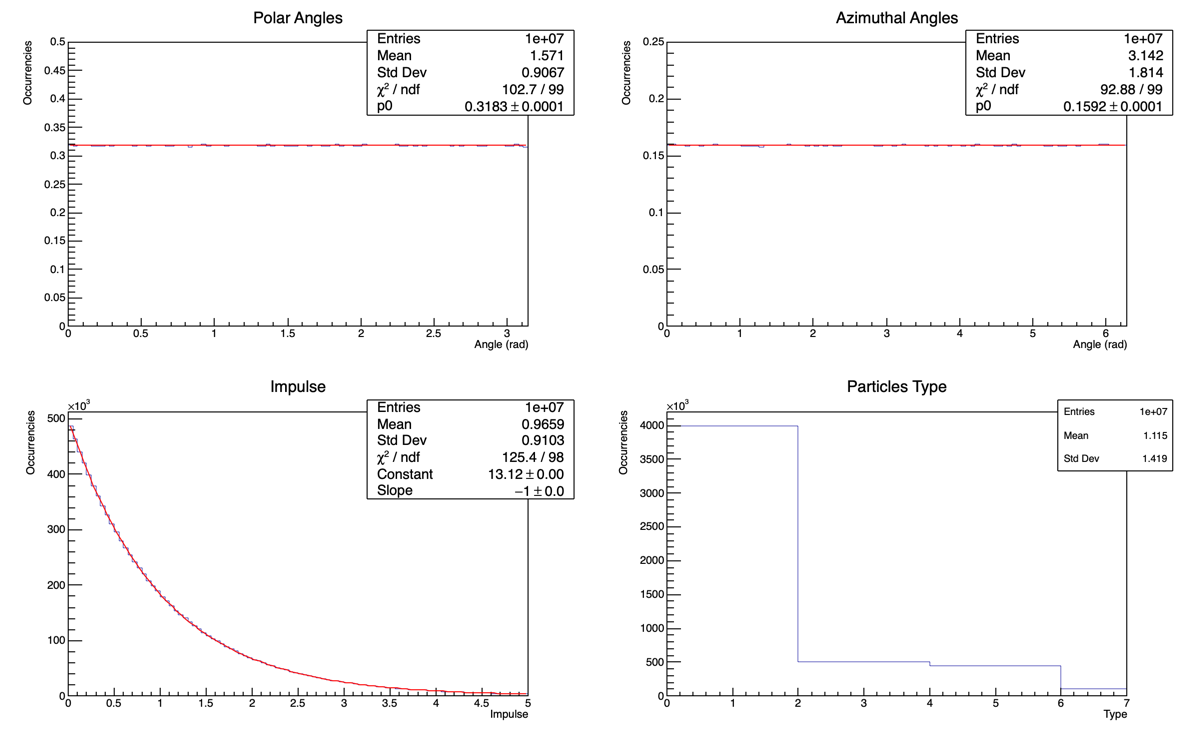
\includegraphics[scale=0.4]{images/DistributionsCanvas.png}

\label{fig:fig1}
\caption{Distribuzioni di angolo polare, angolo azimutale, modulo dell'impulso e tipo di particella}
\end{figure}

\begin{figure}[H]
\centering
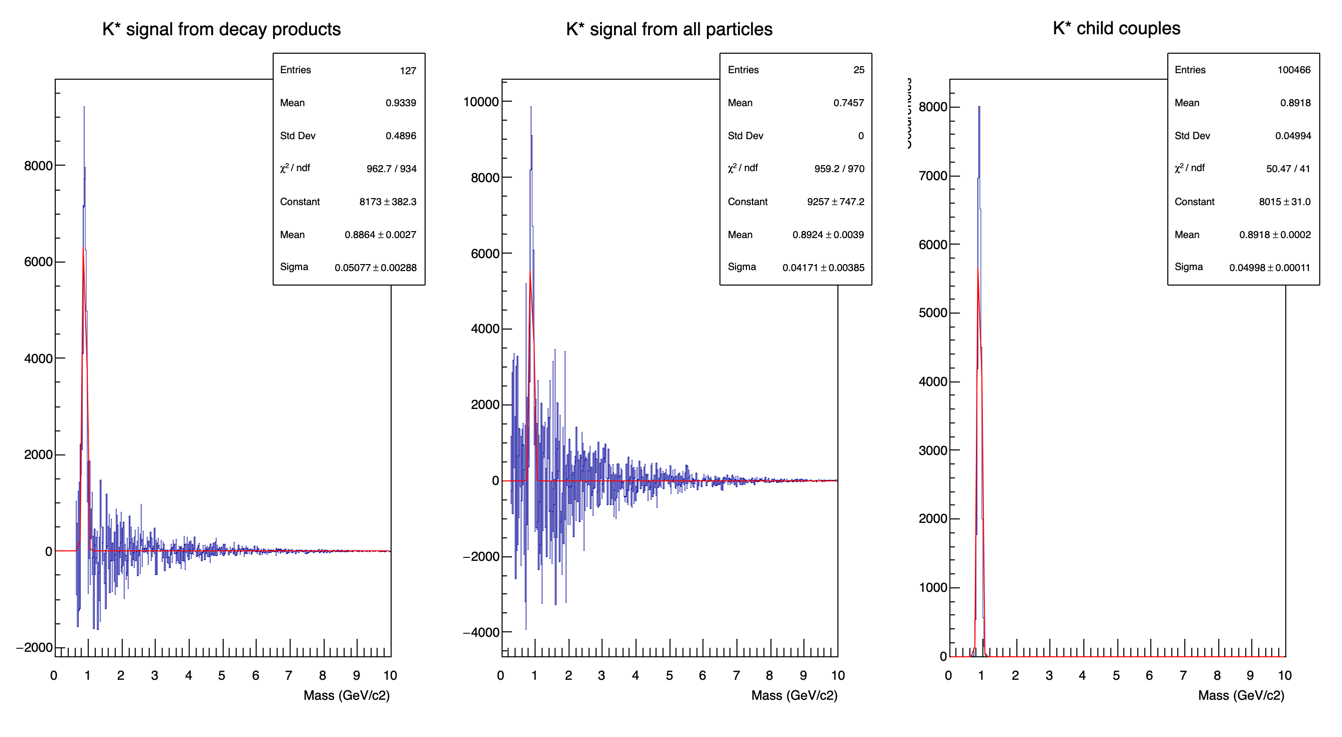
\includegraphics[scale=0.4]{images/SignalCanvas.png}

\label{fig:fig2}
\caption{Distribuzione delle masse invarianti.}
\end{figure}

In figura \ref{fig:fig2} sono riportate le distribuzioni di massa invariante. A sinistra, ottenute per sottrazione degli istogrammi di massa invariante Pioni-Kaoni \textit{discorde-concorde}. Al centro, ottenuti per sottrazione degli istogrammi di massa invariante tra tutte le particelle di carica \textit{discorde-concorde}. A destra, le masse invarianti ottenute a partire dalle particelle figlie di una stessa K*.

\subsection{Consistenza delle distribuzioni}
Le distribuzioni dei parametri cinematici e del tipo di particella (figura \ref{fig:fig1}) sono consistenti con le impostazioni del generatore.


\section{Appendice}



\end{document}